It is important to note that the majority of time in demand paging occurs in
operating system software running in the page-fault handler. The OS must walk
the page tables, look up per-page meta-data in internal data structures, and
allocate a new frame, among other \gls{bookkeeping} tasks (see Section
\ref{sec:linuxImpl} for more details on this process). Our experiments on a
modern x86-based platform found that this processing can take anywhere from
\SIrange{2}{5}{\micro\second}. While this latency is tolerable when accessing a
slow disk (with access latencies on the order of \SI{10}{\milli\second}), it is
a significant overhead when using fast remote memory (with
\SI{1}{\micro\second} access latency) as a backing store. To demonstrate this
effect, we modified the Linux kernel to swap to pre-allocated DRAM buffers in
local memory instead of an external device.  This effectively eliminates
backing store access times and directly measures the overhead of using paging
at all.

\begin{figure}[h]
    \centering
    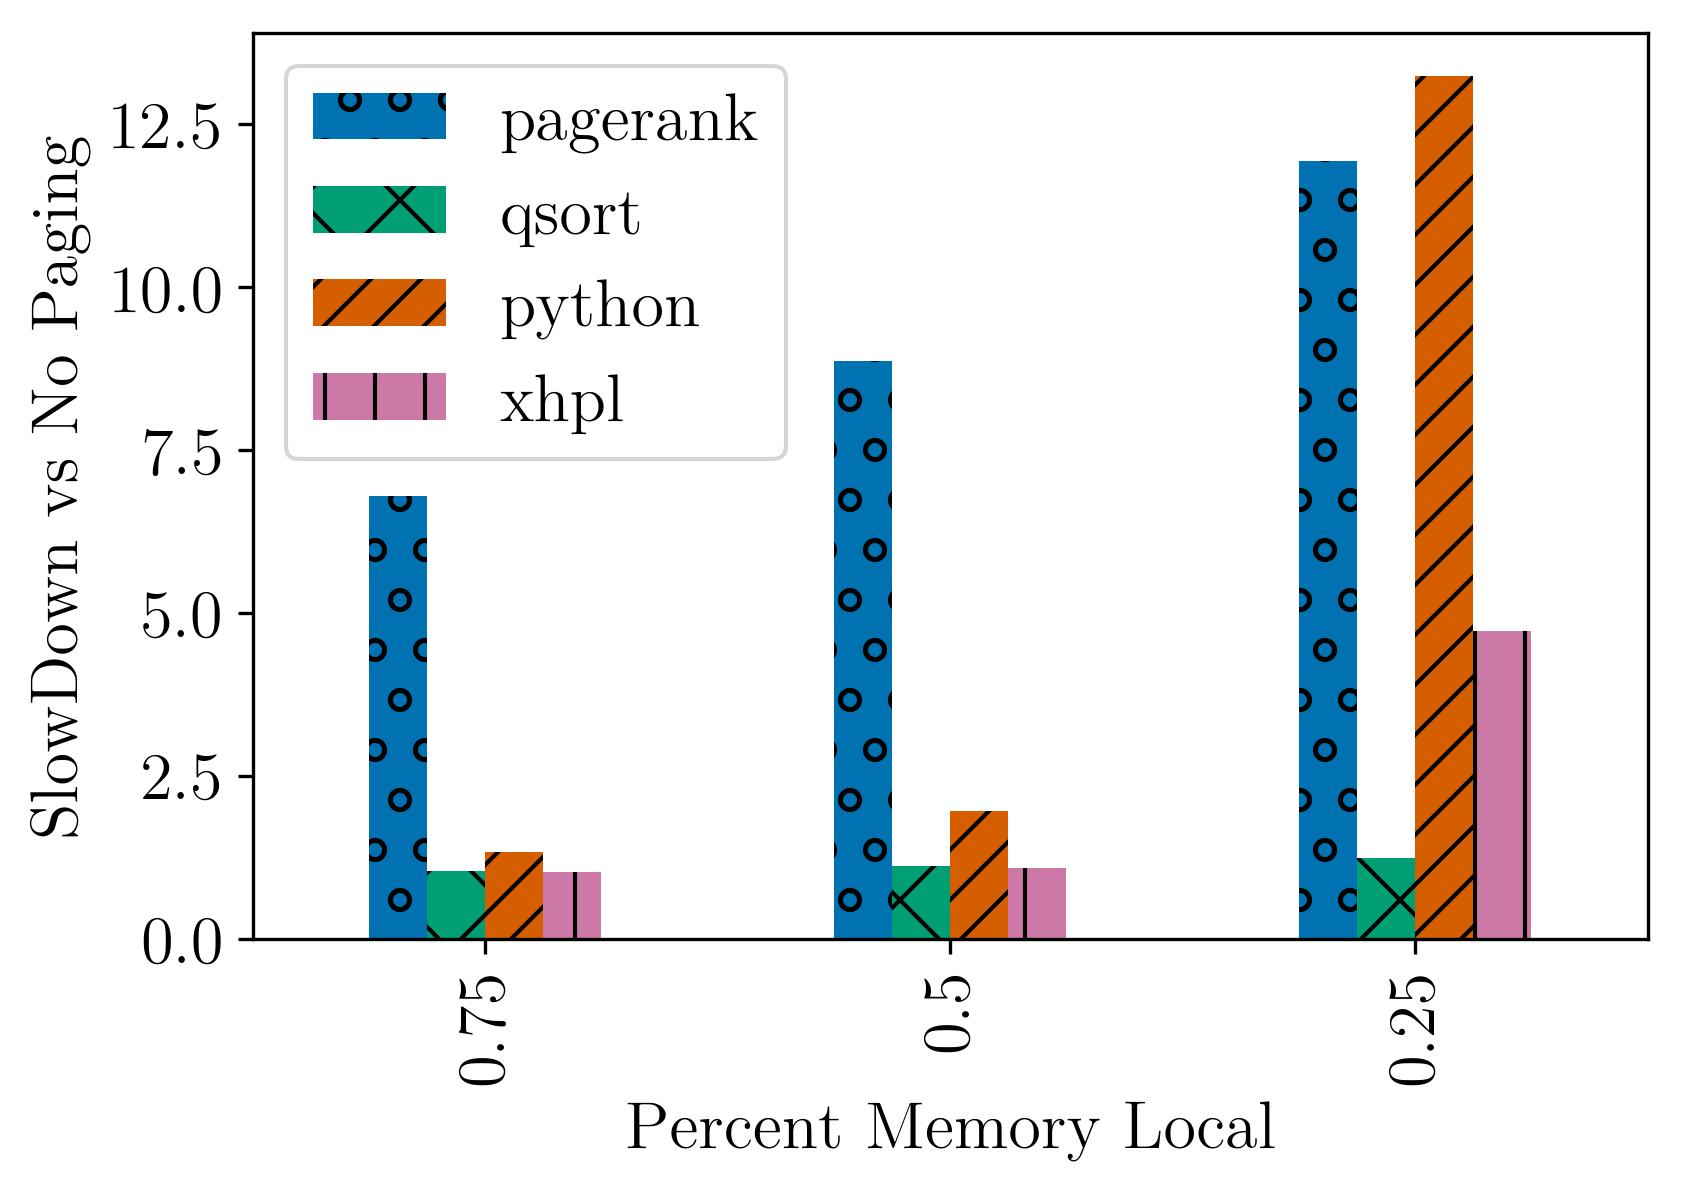
\includegraphics[width=0.9\columnwidth]{figs/paging_overhead.png}
    \caption{Application slow-down when paging to local memory. Memory
oversubscription refers to the percent of peak memory that was stored remotely.}
    \label{fig:paging_overhead}
\end{figure}

Figure \ref{fig:paging_overhead} plots the results of this experiment. Some
applications (such as quicksort or Tensorflow) have good locality and therefor
experience relatively little impact from paging (although even these
applications see slowdowns of as much as 40\%). However, applications with
poor locality (such as Java or linpack) can experience significant slowdowns
(up to 4x in this experiment) due solely to the software overhead of paging. 

\todo[inline]{It would be nice to repeat some of these experiments in Firesim.
With or without that, it would be nice to drill down into the why's a bit more
here. For instance, I could measure total page-fault time, or I could measure
cache-miss behavior.}
